\href{http://2.bp.blogspot.com/-4Qt3-twulCI/URPLqwaiEOI/AAAAAAAAC_M/pnLA9Y7YFyI/s1600/Webkit_Logo.png}{

\includegraphics{http://2.bp.blogspot.com/-4Qt3-twulCI/URPLqwaiEOI/AAAAAAAAC_M/pnLA9Y7YFyI/s1600/Webkit_Logo.png}}WebKit Community talk presented by\nolinebreak\textit{Carlos García Campos}.
\\ WebKit is a layout engine software designed to allow web browsers to render html (is not only on web pages). Become a FLOSS project in 2005 when Apple released the code.
\\ Is used in Mac OS X system framework with Safari, Dashboard, Mail, and many other OS X applications. Also you can find WebKit in\nolinebreakNintendo 3Ds, Kindle and Android.
\\
\\ This project started as a branch of the KHTML and KJS libraries from KDE.
\\
\\
\\ It is a community made ​​up by companies: Apple, Nokia, Google, RIM, Igalia, Samsung.
\\
\\ Because most contributions are made by companies, I want to emphasize that the company that provides more code to WebKit is Google.\nolinebreakIt is strange to see this information on a project controlled by Apple.
\\
\\
\begin{tabular}\href{http://2.bp.blogspot.com/-gi3e--cH8tI/URPfYaz_nUI/AAAAAAAAC_4/uf6iUd0rBtY/s1600/bitergia-webkit.png}{
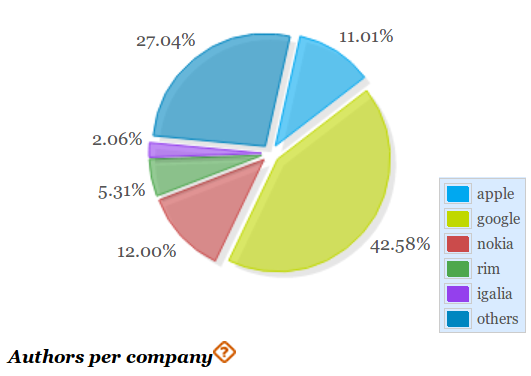
\includegraphics{http://2.bp.blogspot.com/-gi3e--cH8tI/URPfYaz_nUI/AAAAAAAAC_4/uf6iUd0rBtY/s1600/bitergia-webkit.png}} \\ 
\href{http://bitergia.com/public/reports/webkit/2013_01/}{http://bitergia.com/public/reports/webkit/2013\_01/}
\end{tabular} You can see better numbers in the study by Bitergia on WebKit community posted on February 6, 2013, \href{http://blog.bitergia.com/2013/02/06/report-on-the-activity-of-companies-in-the-webkit-project/}{Bitergia blog}.
\\

\subsubsection{ A Foundation, Organization, what is WebKit ?} WebKit is presented as FLOSS project. No reference to any Foundacion as we saw in the case of Apache. So the community living around the project, and any project within the Apache Software Foundation.
\\ WebKit is composed by projects, divided areas for each type of contributor \href{http://www.webkit.org/projects/}{in projects section}.

\subsubsection{ Technologies} documentation :The technologies surrounding the WebKit project, which we consider as ALM Tools, (Application Lifecycle Management) :
\begin{itemize}
	\item Bug Traking System (BTS) Bugzilla -\nolinebreak\href{https://bugs.webkit.org/}{https://bugs.webkit.org/}
	\item Issue Tracking System (ITS) Trac -\nolinebreak\href{http://trac.webkit.org/}{http://trac.webkit.org/}
	\item Early Warning Systems (EWS) Bugzilla -\nolinebreakhttp://webkit-commit-queue.appspot.com/
	\item Developer Guides for each Operative System -\nolinebreak\href{http://www.webkit.org/building/tools.html}{http://www.webkit.org/building/tools.html}
\end{itemize} I will highlight as the \textbf{EWS} tool. \textit{EWS} offers a tracking code contribution we have made to the project (via a patch). It reflects the results of each test in each type of platform. WebKit looks much the appearance of the test because a change can affect millions of users.
\\ As we can see, the system shows a first image of the \href{http://webkit-commit-queue.appspot.com/}{status of contributions}.
\\\href{http://2.bp.blogspot.com/-P50P7P7FyKE/URPW59z7iJI/AAAAAAAAC_c/SKhRknuSaBo/s1600/webkit-queue-status.png}{
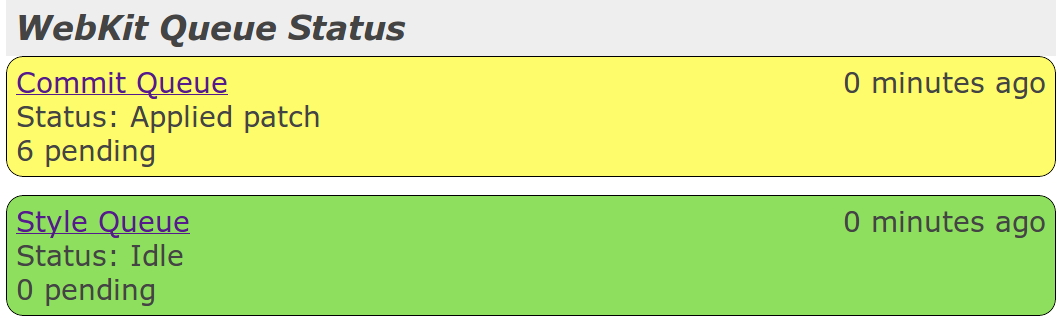
\includegraphics{http://2.bp.blogspot.com/-P50P7P7FyKE/URPW59z7iJI/AAAAAAAAC_c/SKhRknuSaBo/s640/webkit-queue-status.png}}
\\ Accessing \href{http://build.webkit.org/console}{BuildBot WebKit Console}, we have access to the results and follow-up of each of the patches and tests for each of the existing distributions (ports).
\\\href{http://1.bp.blogspot.com/-_fnhPmtRGHQ/URPXRDTyhdI/AAAAAAAAC_k/d08LrFTOWZ8/s1600/webkit-build-bot.png}{
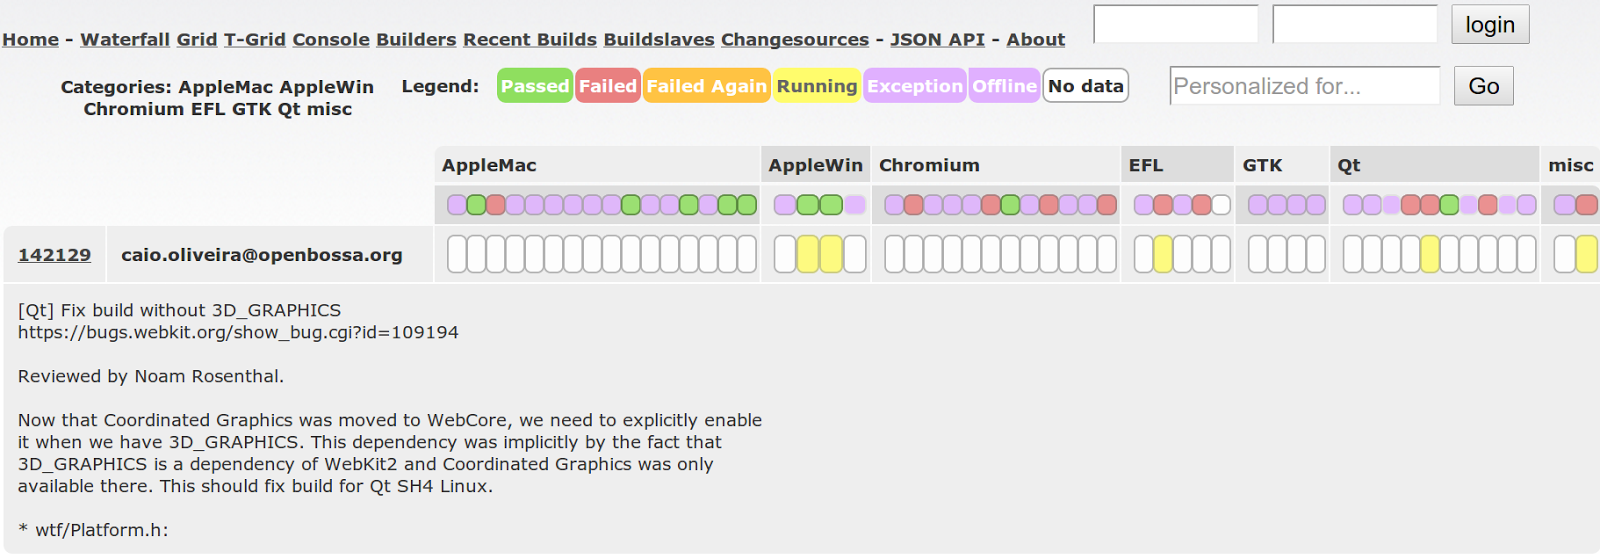
\includegraphics{http://1.bp.blogspot.com/-_fnhPmtRGHQ/URPXRDTyhdI/AAAAAAAAC_k/d08LrFTOWZ8/s640/webkit-build-bot.png}}
\\ It is very rigorous system of contributions to the project, we will see in the next section.
\\ WebKit has a very useful\nolinebreak\nolinebreakdevelopment guidelines documentation:
\begin{itemize}
	\item \textit{Coding style guidelines} - http://www.webkit.org/coding/coding-style.html
	\item \textit{Technical Articles} - http://www.webkit.org/coding/technical-articles.html
	\item \textit{Regression Testing} - http://www.webkit.org/quality/testing.html
	\item \textit{Reporting Bugs} - http://www.webkit.org/quality/reporting.html
	\item \textit{Bug Life Cycle} - http://www.webkit.org/quality/lifecycle.html
	\item \textit{Wiki Documentation} - http://trac.webkit.org/wiki
\end{itemize}

\subsubsection{ How can I contribute ?} In WebKit there are many ways of contributions; translations, code, documentation, etc. We are going to focus on contribute with code.
\\ There is a guideline explaining \href{http://www.webkit.org/coding/contributing.html}{how to contribute code}. These are the steps you have to follow to contribute code in WebKit:
\begin{itemize}
	\item Choose or create a bug report to work on.
	\item Develop your changes.
	\item Make sure your changes meet the code style guidelines. The check-webkit-style script may be of help.
	\item Run the layout tests using the run-webkit-tests script and make sure they all pass. See the testing page for more information, as well as what you need to do if you've modified JavaScriptCore.
	\item Add any new files to your working directory.
	\item Prepare a change log entry. You may have to add entries to multiple ChangeLogs. The prepare-ChangeLog script will create stub entries for you. See the paragraph about ChangeLogs below.
	\item Create the patch using the svn-create-patch script.
	\item Submit your patch for review to bugs.webkit.org.
	\item Make any changes recommended by the reviewer.
	\item Once reviewed, ask someone to land your patch or mark it for automated commit.
	\item Please watch for any regressions it may have caused (hopefully none)!
\end{itemize}

\subsubsection{ Committers and Reviewers} WebKit contributors are divided into two groups; \textit{committers} and \textit{reviewers}. The committers can contribute code to\nolinebreakthe reviewers agree.
\\\textit{To be a committer}, you have to be nominated by the reviewers. Having a minimum number of significant patches \textit{(ranges between 10 and 20)}. Bureaucratic process and receive approval of 3. Is searching the plurality of contacting between one or more reviewers.
\begin{quotation}\textit{Any company with more than three reviewers may give permission to a reviewer.}
\end{quotation} Becoming reviewer, is a higher jump. You have been elected by \textit{reviewers from different companies and have contributed over 80 functional patches}.
\\ Both steps are accompanied by the signing of an agreement with Apple, not with the WebKit project.
\\
\\\textit{I Hope you enjoy reading this information and\nolinebreakI recommend watching the video presentation.}